\documentclass{scrartcl}
\usepackage[utf8]{inputenc}
\usepackage[T1]{fontenc}      
\usepackage[francais]{babel}
% Layout and figures
%\usepackage[top=2.5cm,bottom=2.5cm,right=2.5cm,left=2.5cm]{geometry}
\usepackage{subfigure}
\usepackage{rotating}
% Math
\usepackage{amsmath}
\usepackage{amssymb}
\usepackage{amsthm}
\usepackage{float}
% Links
\usepackage{url}
\usepackage{hyperref}
\hypersetup{
    colorlinks,
    citecolor=black,
    filecolor=black,
    linkcolor=black,
    urlcolor=black
}
% New commands
\newcommand{\annexe}{\part{Annexes}\appendix}
\newcommand{\biblio}[1]{\bibliographystyle{plain}\bibliography{#1}\nocite{*}}

\newcommand{\doctitle}[1]{
	\title{LSINF1225 - Projet BarTender}
	\subtitle{#1}
	\author{\textbf{Groupe T}\\
	\textsc{Gérard} Louis (6317-12-00)\\
	\textsc{Gillon} Bastien (5937-12-00)\\
	\textsc{Jacques} Thibault (2954-13-00)\\
	\textsc{Paris} Antoine (3158-13-00)\\
	\textsc{Ramelot} Sylvain (4763-13-00)}
	\date{\today}

	\begin{document}

	\maketitle
	%\tableofcontents
}

\doctitle{BarTender : présentation du prototype}

\section{Manuel d'utilisation}
\subsection{Écran d'accueil de l'application}
Lorsque l'application démarre, vous accédez à l'écran
présenté sur la figure \ref{fig:main-menu}. Sur cet écran,
il est possible d'accéder à la carte, de se connecter ou de
s'inscrire.

\begin{figure}[H]
	\centering
	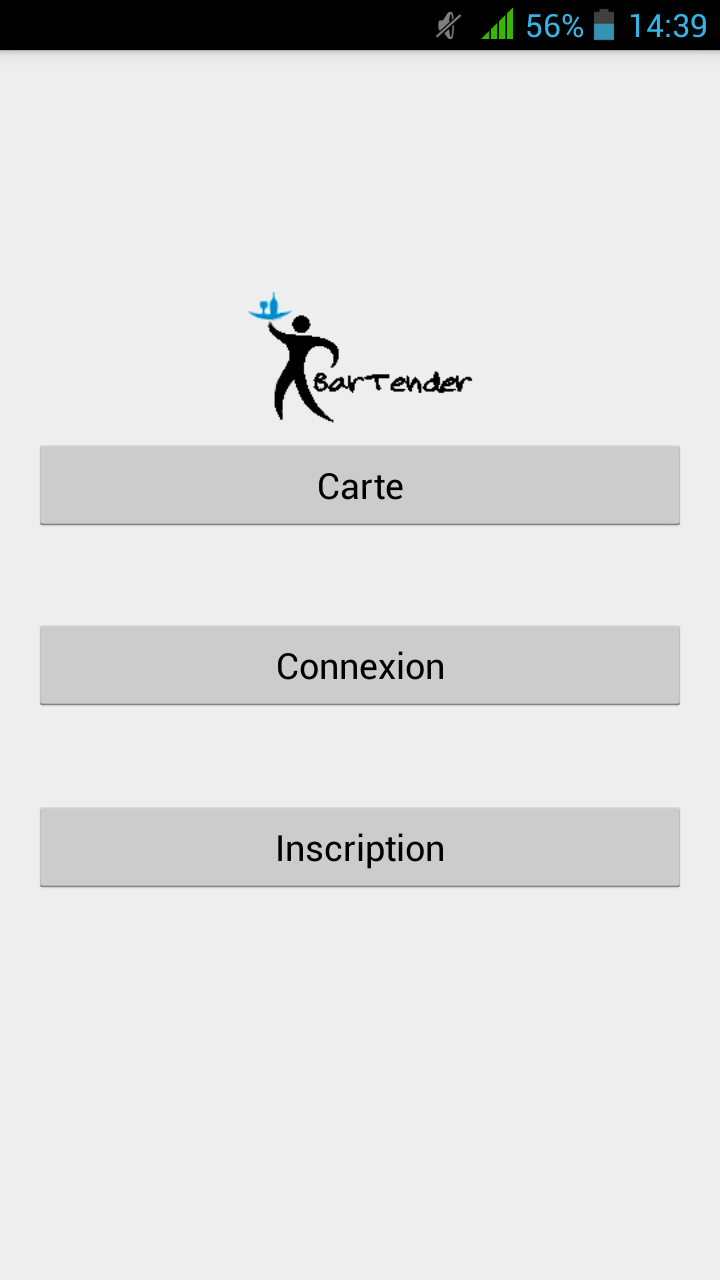
\includegraphics[scale=0.15]{img/main-menu.png}
	\caption{Écran d'accueil de l'application.}
	\label{fig:main-menu}
\end{figure}

\subsection{Connexion et inscription}
Pour se connecter à l'application, il suffit de cliquer
sur le bouton ``Connexion'' de l'écran d'accueil. Vous
arrivez alors sur un écran similaire à la figure \ref{fig:register-login}
sur lequel il vous suffit d'indiquer votre identifiant et votre
mot de passe. Pour s'inscrire sur l'application, il suffit de cliquer
sur le bouton ``Inscription'' de l'écran d'accueil. Vous arrivez alors à un écran similaire à la figure \ref{fig:register-login}. L'inscription
est volontairement simple et ne demande qu'un identifiant, un mot
de passe et sa confirmation. 

\begin{figure}[H]
    \centering
    \begin{subfigure}
				\centering
				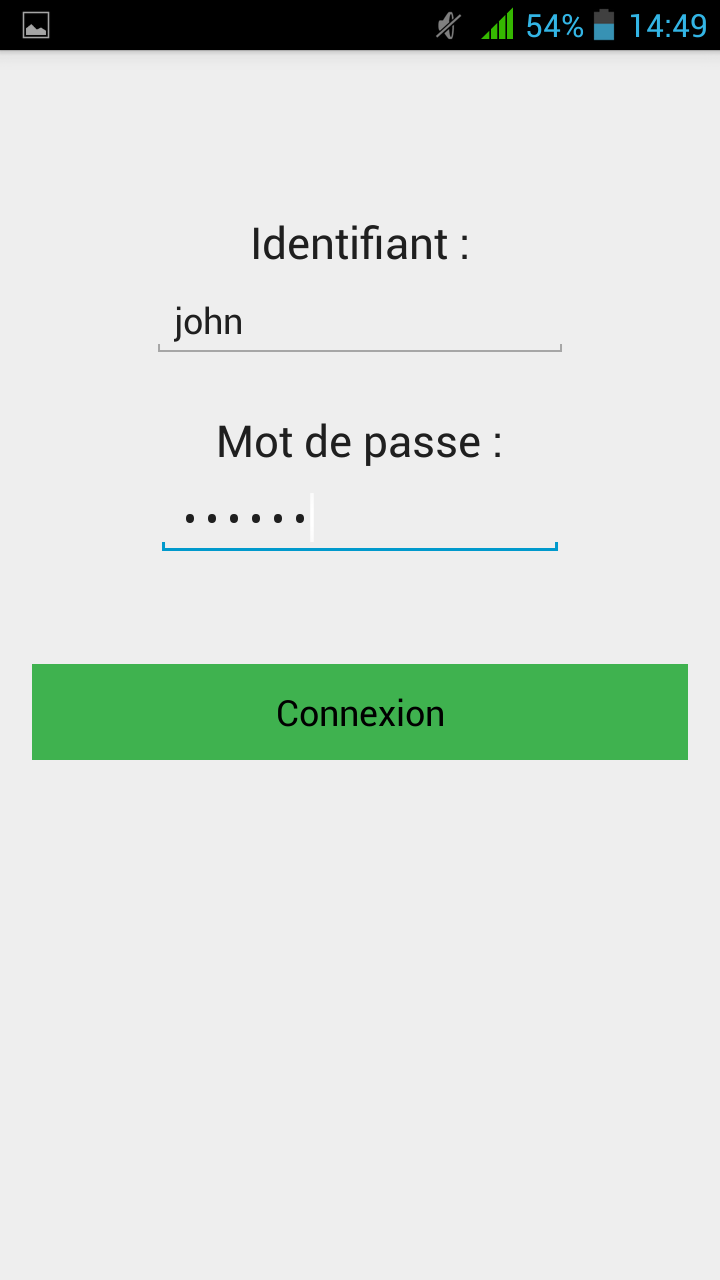
\includegraphics[scale=0.15]{img/login.png}
    \end{subfigure}%
    ~ 
    \begin{subfigure}
				\centering
				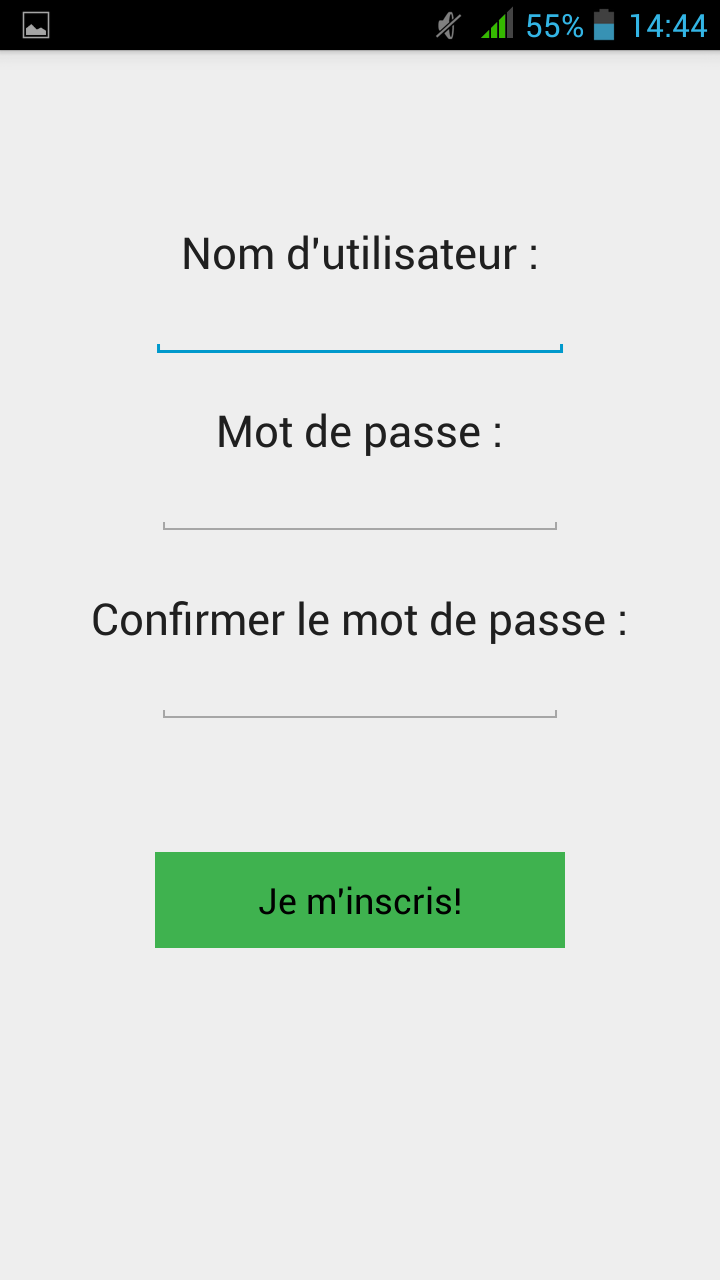
\includegraphics[scale=0.15]{img/register.png}
		\end{subfigure}
    \caption{Page de connexion à gauche, et d'inscription à droite.}
		\label{fig:register-login}
\end{figure}

\subsection{La carte}
La carte est accessible de plusieurs manières. Premièrement, depuis l'écran d'accueil
présenté à la figure \ref{fig:main-menu}. Ce bouton permet à un client qui ne désire
pas créer un compte de quand même pouvoir consulter la carte. Bien évidemment, la carte
est également accessible une fois connecté. La carte se présente comme sur la
figure \ref{fig:carte}. Il est possible de trier les boissons par noms ou par prix,
en cliquant respectivement sur ``Boisson'' ou ``prix''.

\begin{figure}[H]
	\centering
	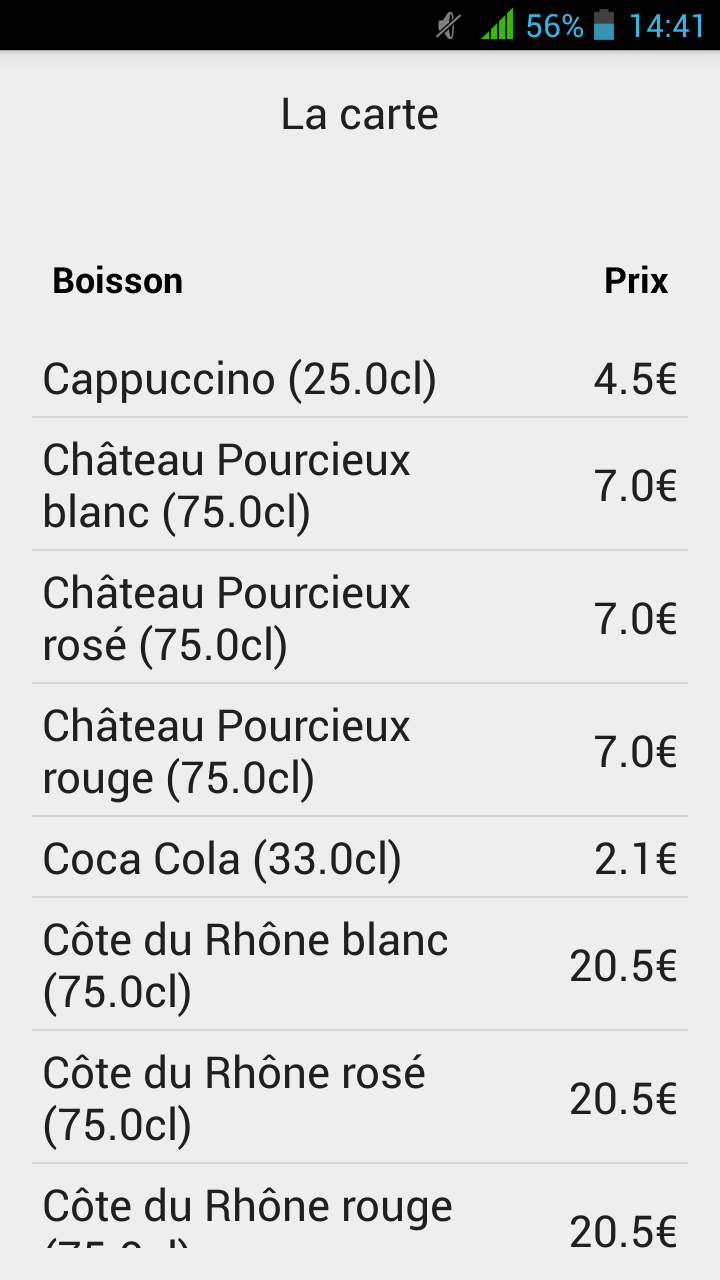
\includegraphics[scale=0.15]{img/carte.png}
	\caption{Carte des boissons.}
	\label{fig:carte}
\end{figure}

En cliquant sur une boisson, des détails apparaissent. Ces détails sont bien
sur différents selon que vous soyez connecté en tant que client ou en tant
que serveur. Pour chaque boisson, le client pourra lire une courte
description, un volume, un prix et une note moyenne (donnée par d'autres
clients), comme présenté sur la figure \ref{fig:drink-details}.

\begin{figure}[H]
	\centering
	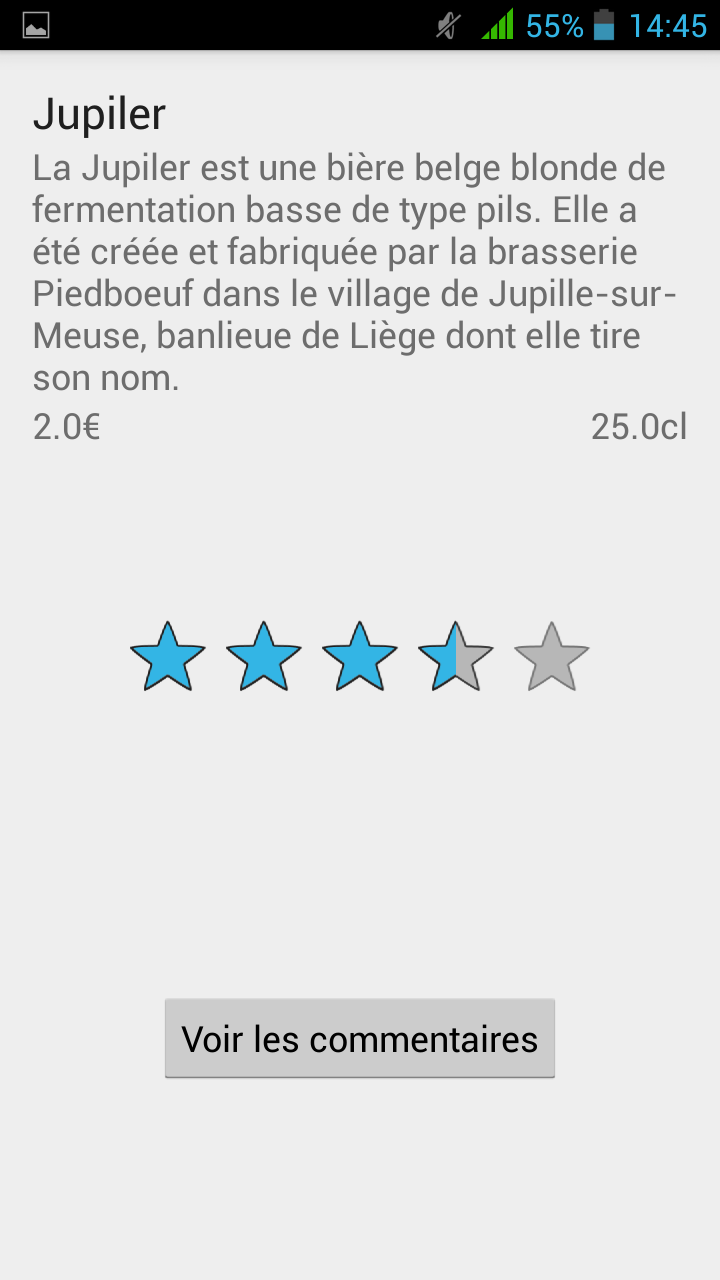
\includegraphics[scale=0.15]{img/drink-details.png}
	\caption{Détails d'une boisson.}
	\label{fig:drink-details}
\end{figure}

Pour un serveur, ces détails sont un peu différents. Ils contiennent
cette fois des informations sur le stock des boissons : le stock
actuel, le stock maximum, et le seuil minimal (indiquant qu'il est temps
de recommander cette boisson auprès du fournisseur). Ces informations
sont représentés de façon plus visuelle dans une barre d'évolution.

\begin{figure}[H]
    \centering
    \begin{subfigure}
        \centering
        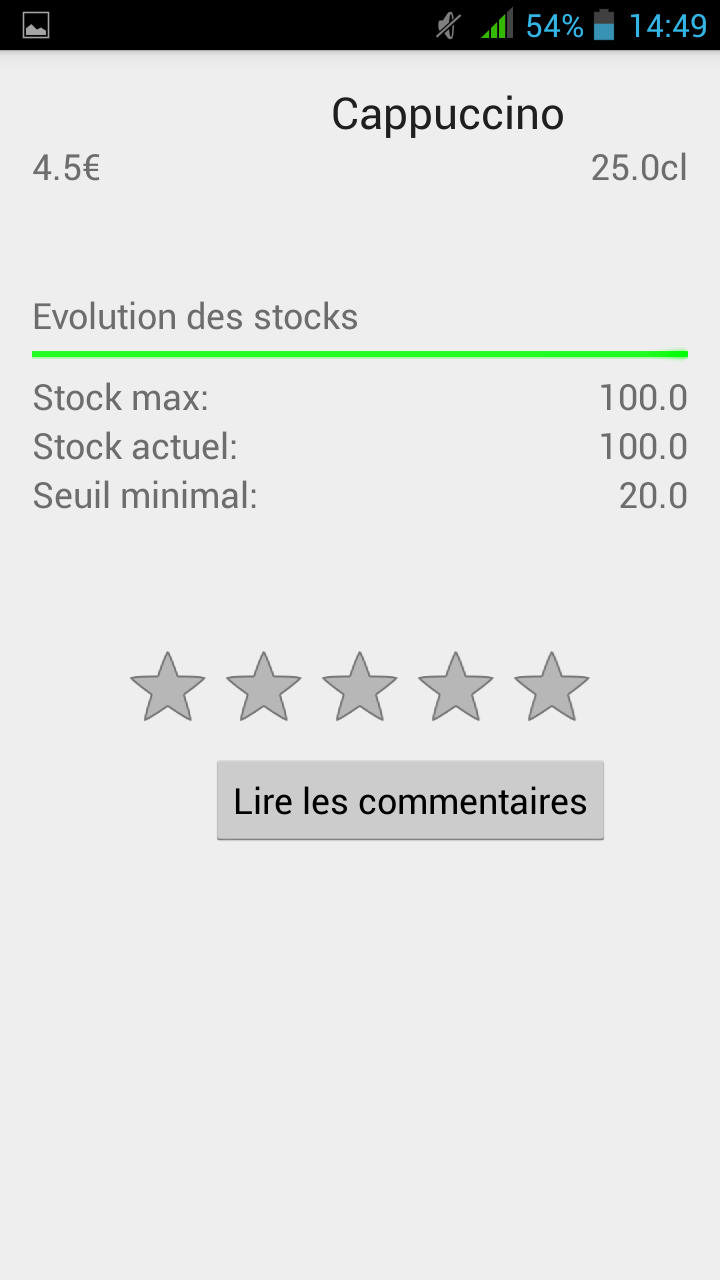
\includegraphics[scale=0.15]{img/stock-full.png}
    \end{subfigure}%
    ~ 
    \begin{subfigure}
        \centering
        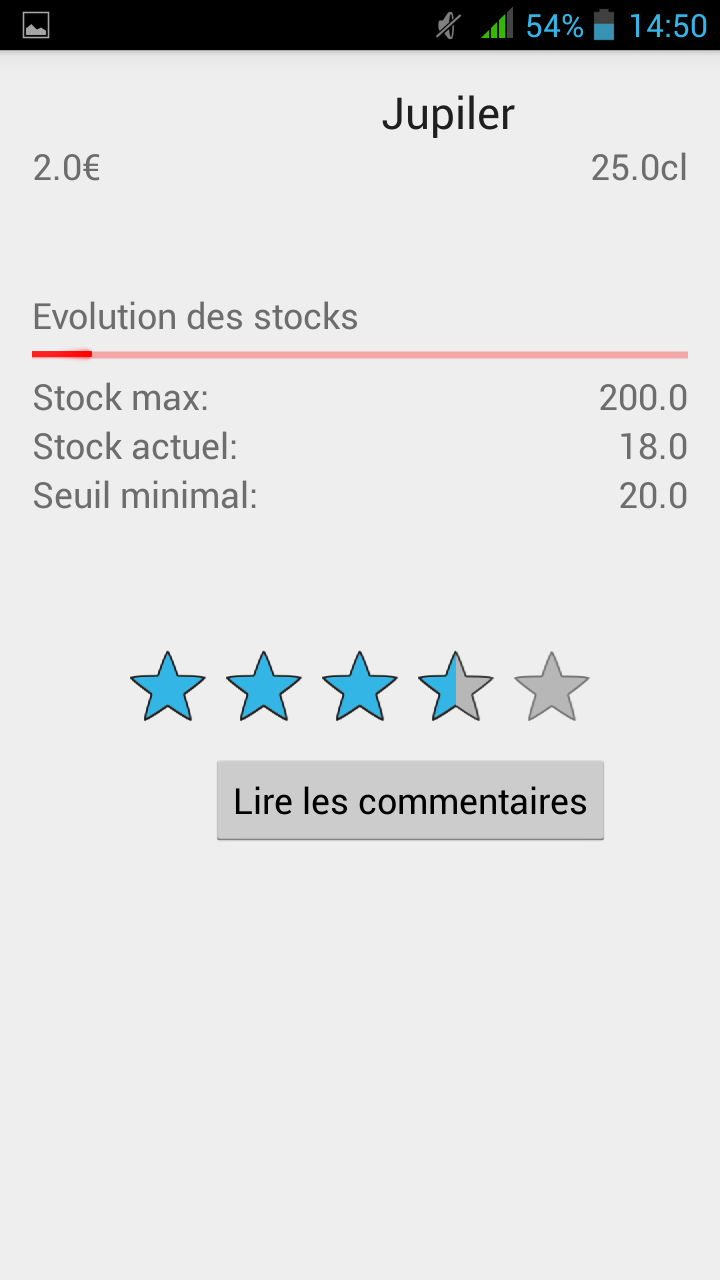
\includegraphics[scale=0.15]{img/stock-empty.png}
    \end{subfigure}
    \caption{Détails d'une boisson côté serveur.}
		\label{fig:stocks}
\end{figure}

Comme le montre la figure \ref{fig:stocks}, la couleur de cette barre
change selon que l'on soit en-dessous ou au-dessus du seuil minimal.

\subsection{La recherche avancée}
Le client et le serveur ont tous les deux accès à une fonctionnalité commune,
la recherche avancée, présentée sur la figure \ref{fig:search}. 
Différents critères de recherches sont disponibles : par nom, par catégorie
et sous-catégorie, et en indiquant un prix mimimum et maximum.

\begin{figure}[H]
	\centering
	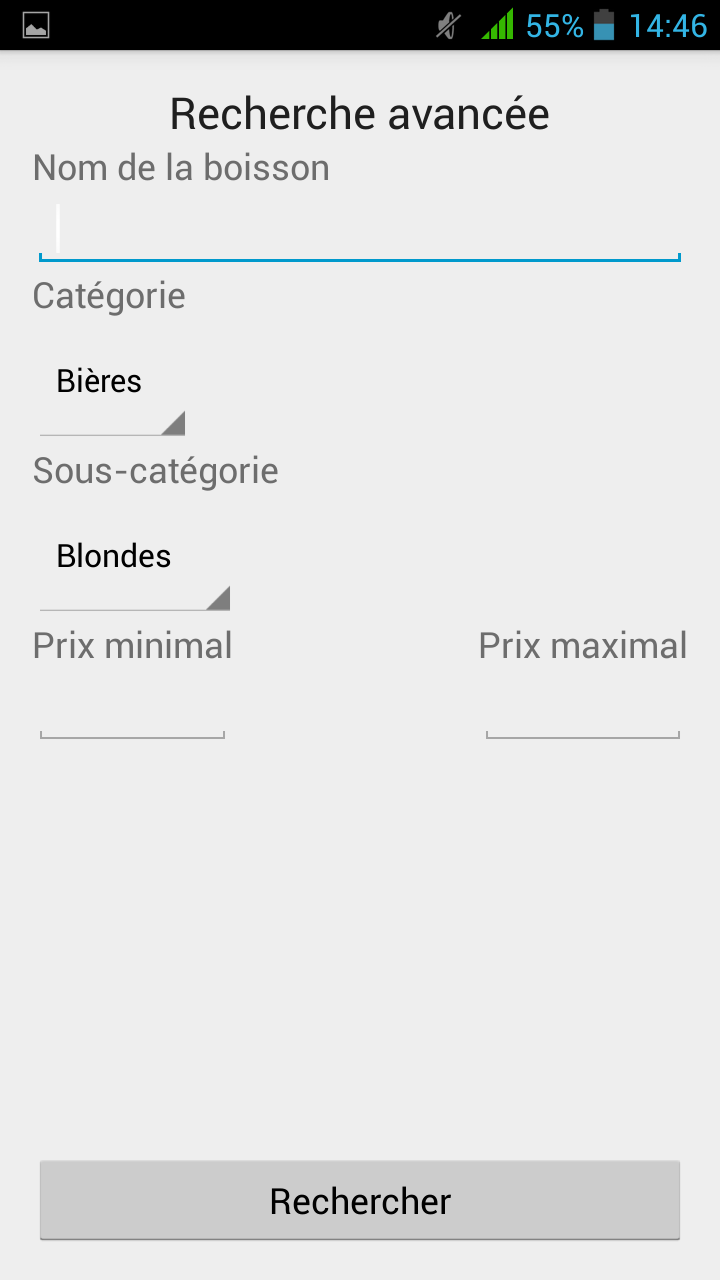
\includegraphics[scale=0.15]{img/search.png}
	\caption{Recherche avancée.}
	\label{fig:search}
\end{figure}

\subsection{Passer une commande}
Le serveur est la seul personne à pouvoir passer une commande. Un fois connecté, celui ci peut cliquer sur le button "Commande" dans son menu pour passer une commande pour une table. Une page avec tous les commandes va lui être proposé.

\begin{figure}[H]
    \centering
    \begin{subfigure}
        \centering
        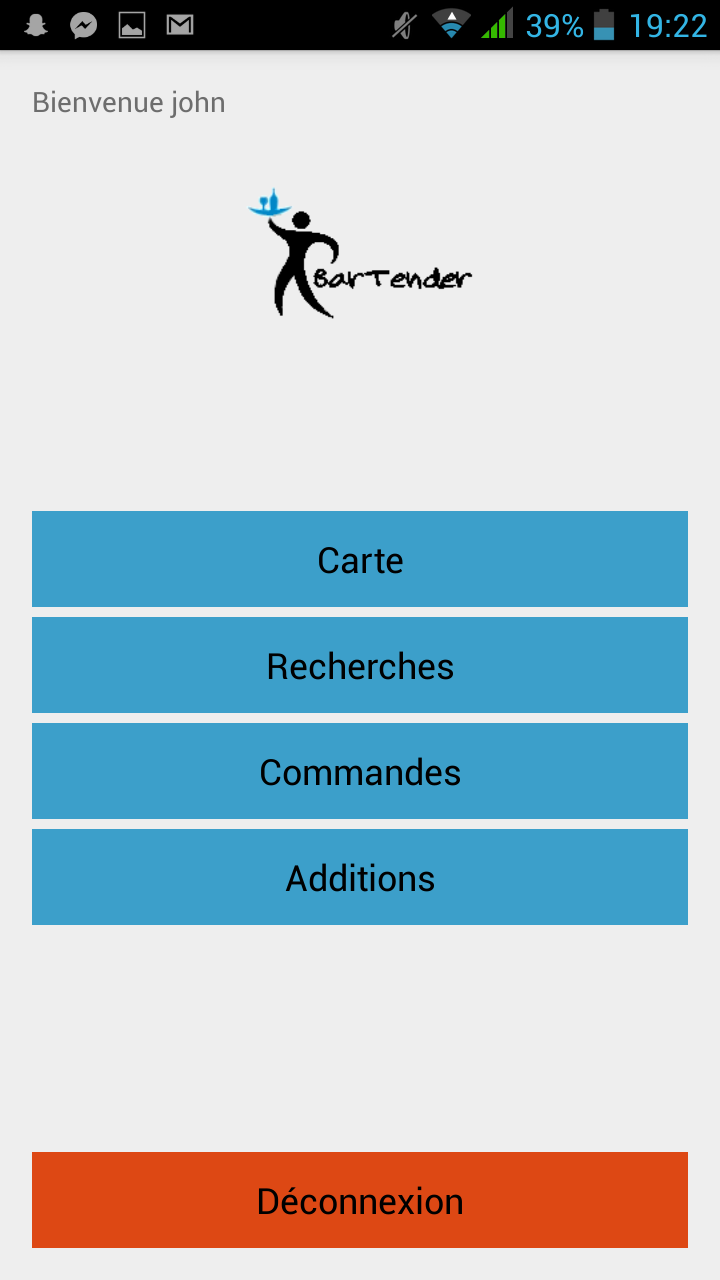
\includegraphics[scale=0.15]{img/waiter-logged.png}
    \end{subfigure}%
    ~ 
    \begin{subfigure}
        \centering
        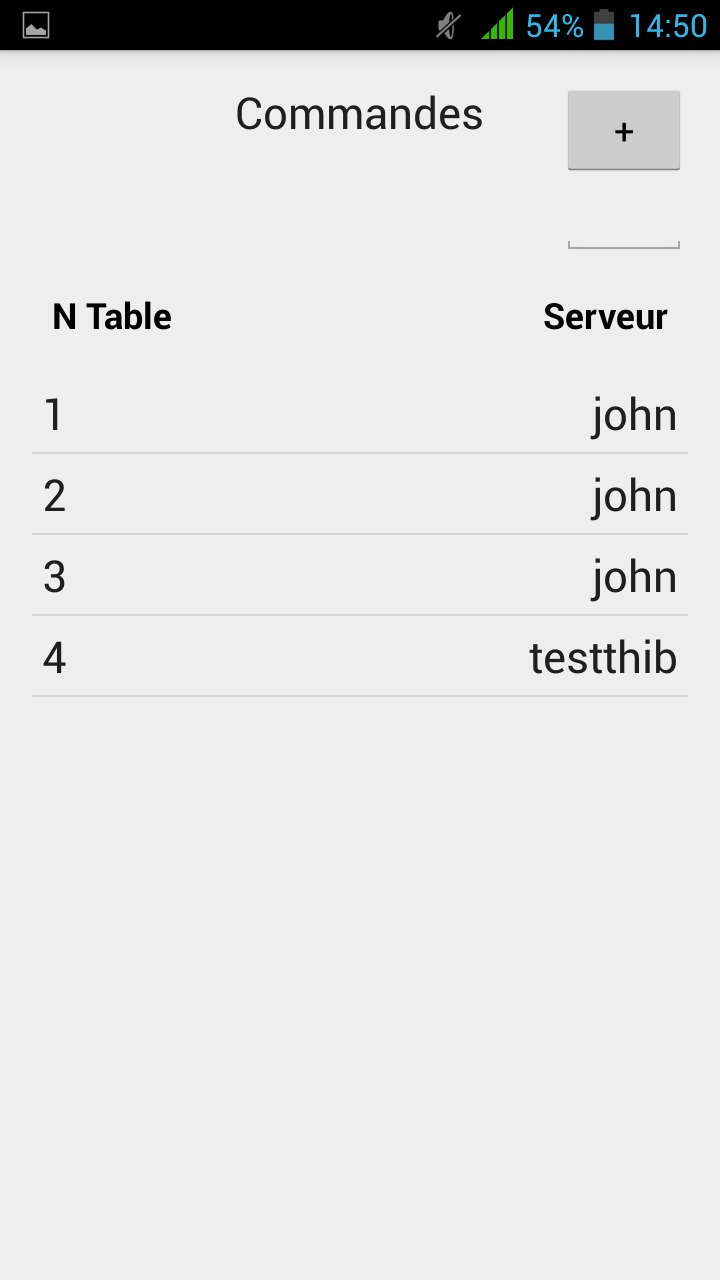
\includegraphics[scale=0.15]{img/orders.png}
    \end{subfigure}
    \caption{Menu du serveur et liste de commandes.}
    \label{fig:Menu-server}
\end{figure}

Le serveur sélectionne le numero de table pour laquel il va passer commande et après confirmation du numero de table, la carte va s'ouvrir. Il choissit la boisson en cliquant dessus et donne la quantité de boissons à commander. 

\begin{figure}[H]
	\centering
	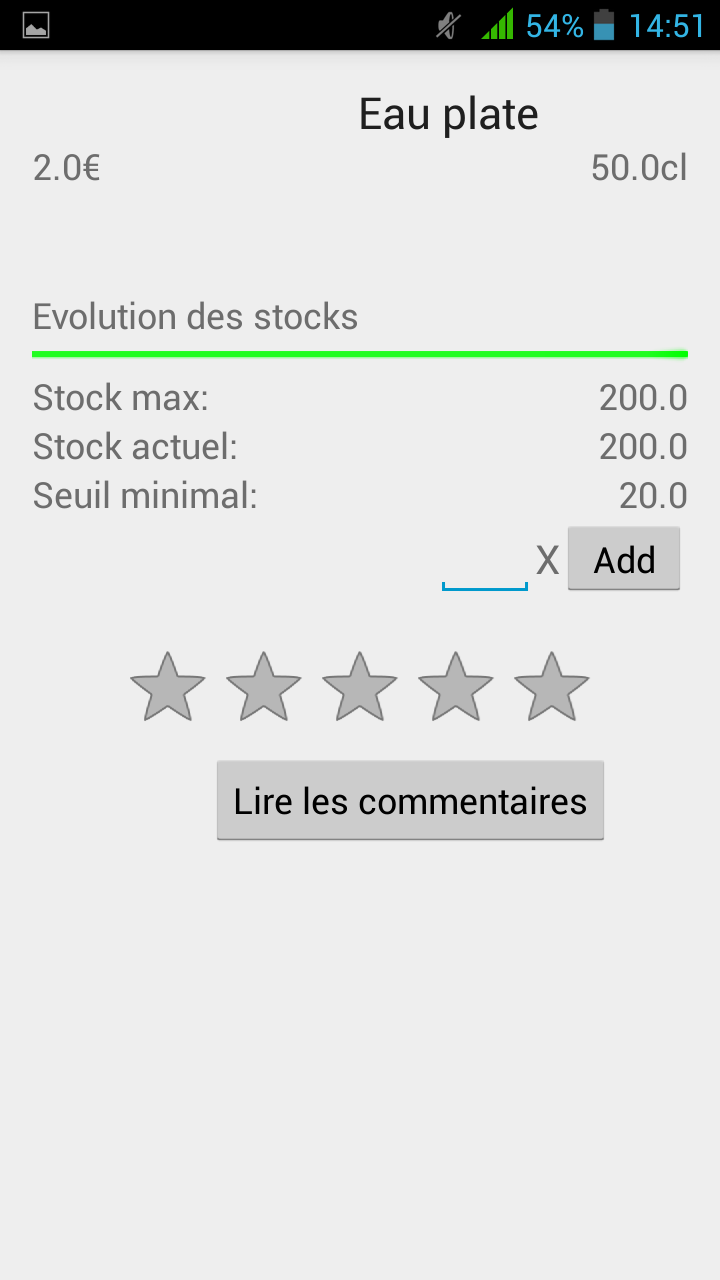
\includegraphics[scale=0.15]{img/add-drink.png}
	\caption{Ajout d'une boisson}
	\label{fig:add-drink}
\end{figure}

Une fois toutes les boissons commandées, le serveur appuie sur le bouton 'Finir commande' pour terminer la commande pour cette table. Il sera renvoyer sur le menu des commandes.

\begin{figure}[H]
	\centering
	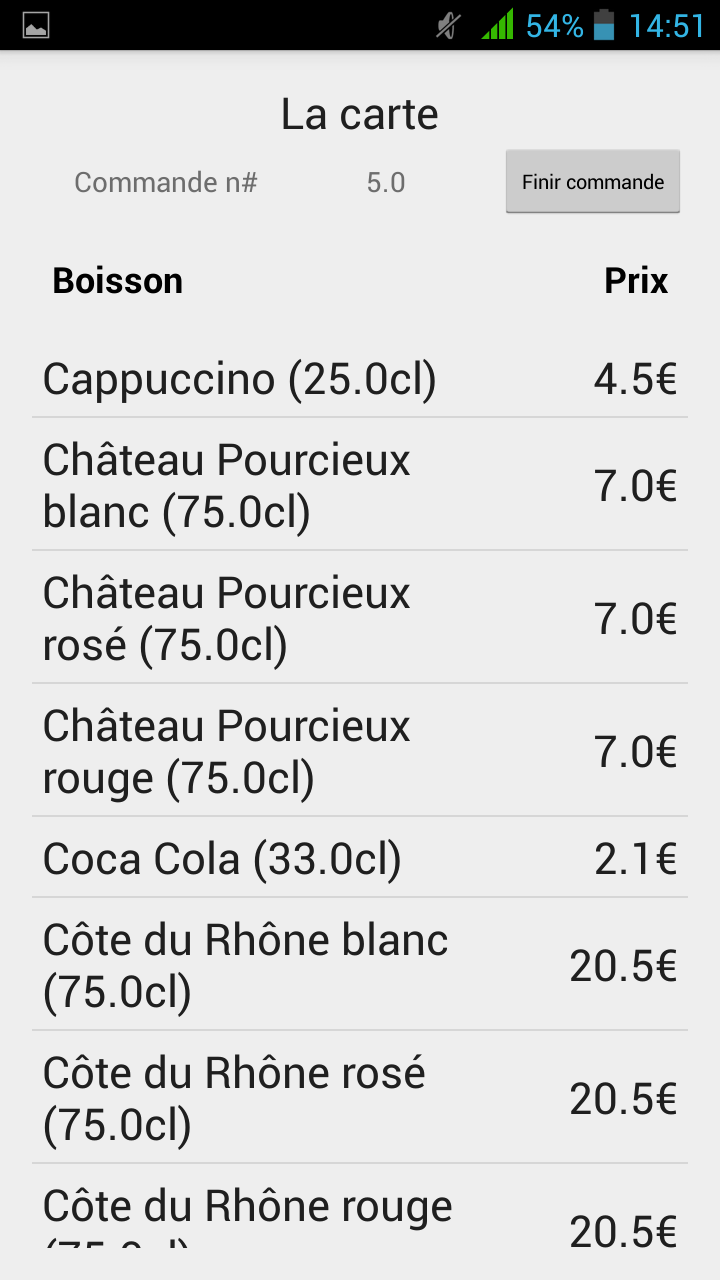
\includegraphics[scale=0.15]{img/new-order.png}
	\caption{Carte pour ajouter des boissons à une commande}
	\label{fig:drink-list}
\end{figure}

\subsection{Créer une addition}
Une fois une commande passée, il est possible de crée un addition à partir d'un numero de table. Une fois le serveur connecté, il appuie sur le button "Addition" de son menu. Le menu d'addition est une liste des additions en cours. Pour en crée une nouvelle, il appuie sur le button "+" qui va lui proposer plusieurs numeros de tables qui ont des commandes en cours. Il sélectionne une table, confirme et une nouvelle addition sera crée.

\begin{figure}[H]
	\centering
	\begin{subfigure}
		\centering
		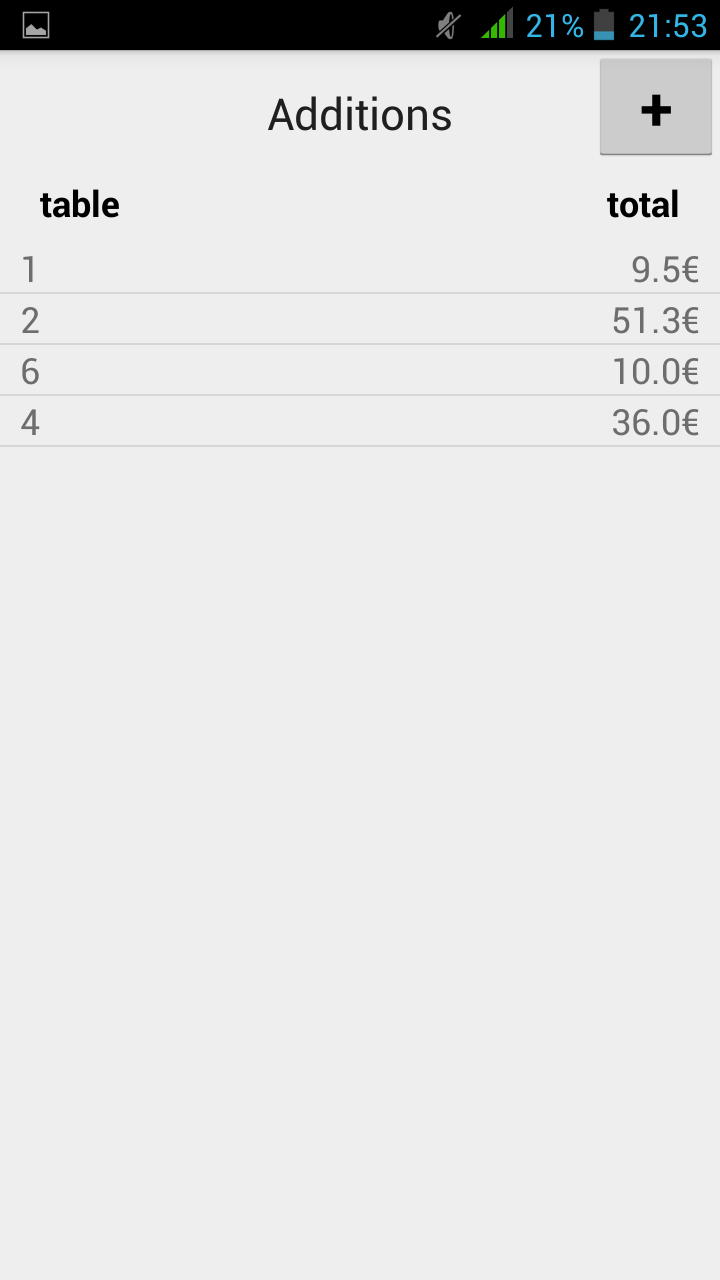
\includegraphics[scale=0.15]{img/bills-list.png}
	\end{subfigure}%
	~
	\begin{subfigure}
		\centering
		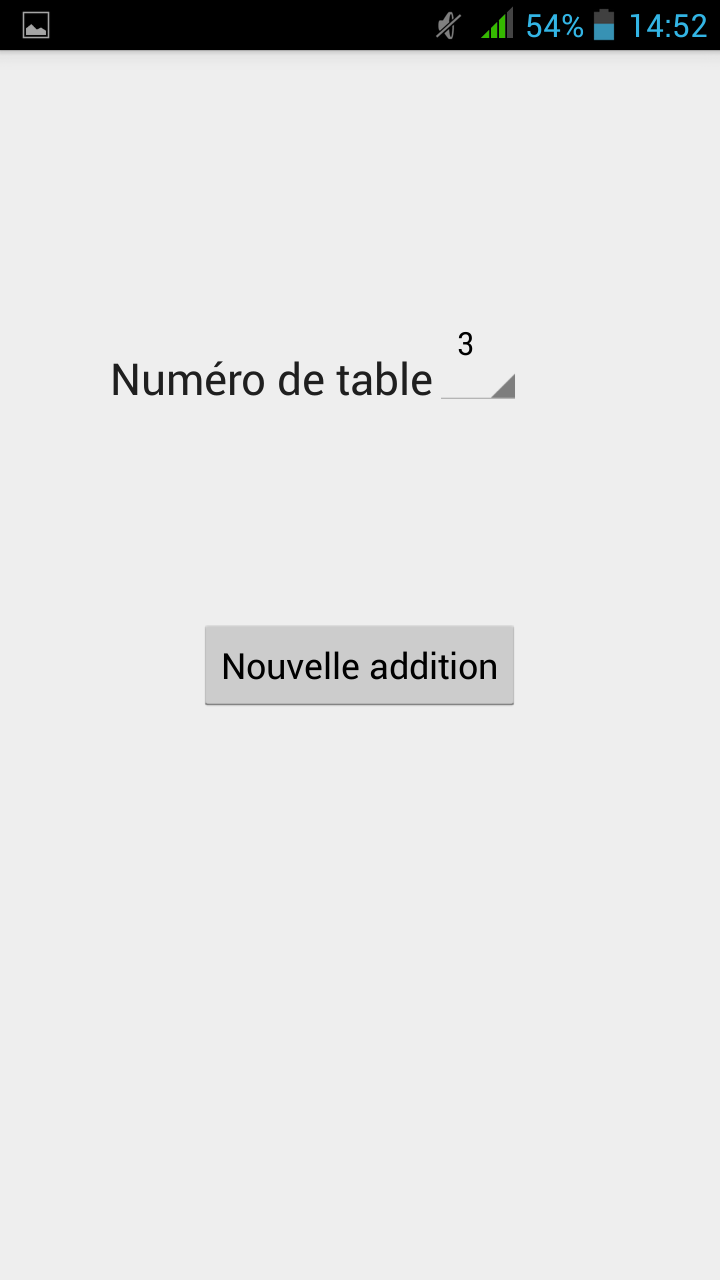
\includegraphics[scale=0.15]{img/new-bill.png}
	\end{subfigure}
	\caption{List des additions \& Nouvelle addition}
\end{figure}

Pour voir les details d'une addition, il suffit de cliquer sur une addition. Une liste de tous les commandes associées à cette addition vont apparaître. Cliquer sur une commande pour avoir plus de détail de celle ci.


\subsection{Cloturer un addition}
Pour cloturer une addition, il suffit d'en sélectionner une et de cliquer sur le button "Cloturer l'addition" pour finir une addition.

\begin{figure}[H]
	\centering
	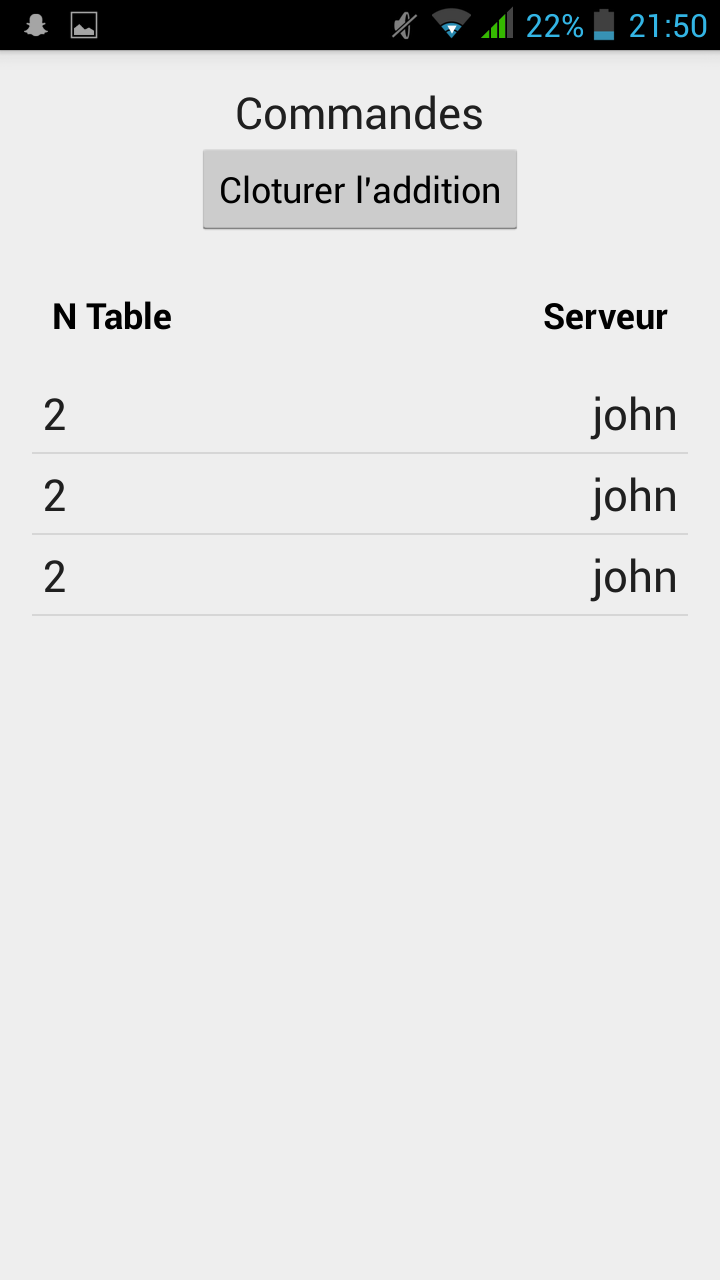
\includegraphics[scale=0.15]{img/details-bill.png}
	\caption{Detail d'une addition}
	\label{fig:bill-details}
\end{figure}

\end{document}